\newpage
\section{Architettura}
\subsection{Metodo e formalismo}
Nell’esposizione dell’architettura dell’applicazione si procederà con un approccio \textit{top-down\ped{G}}, descrivendo l’architettura dal generale al particolare. Si procederà quindi alla descrizione dei \textit{packages\ped{G}} e dei componenti, per poi descrivere nel dettaglio le singole classi, specificando per ognuna il tipo, l’obiettivo, la funzione, relazioni in ingresso e uscita e i metodi e attributi contenuti. Successivamente verranno riportati i diagrammi di sequenza delle principali funzionalità di \progetto, seguendo il formalismo del linguaggio \textit{UML\ped{G}} 2.0. Vengono infine presentati in dettaglio i \textit{design pattern\ped{G}} utilizzati nelle varie parti dell'applicazione.
\subsubsection{Informazioni generali}
\label{Architettura}
\begin{figure}[ht]
	\centering
	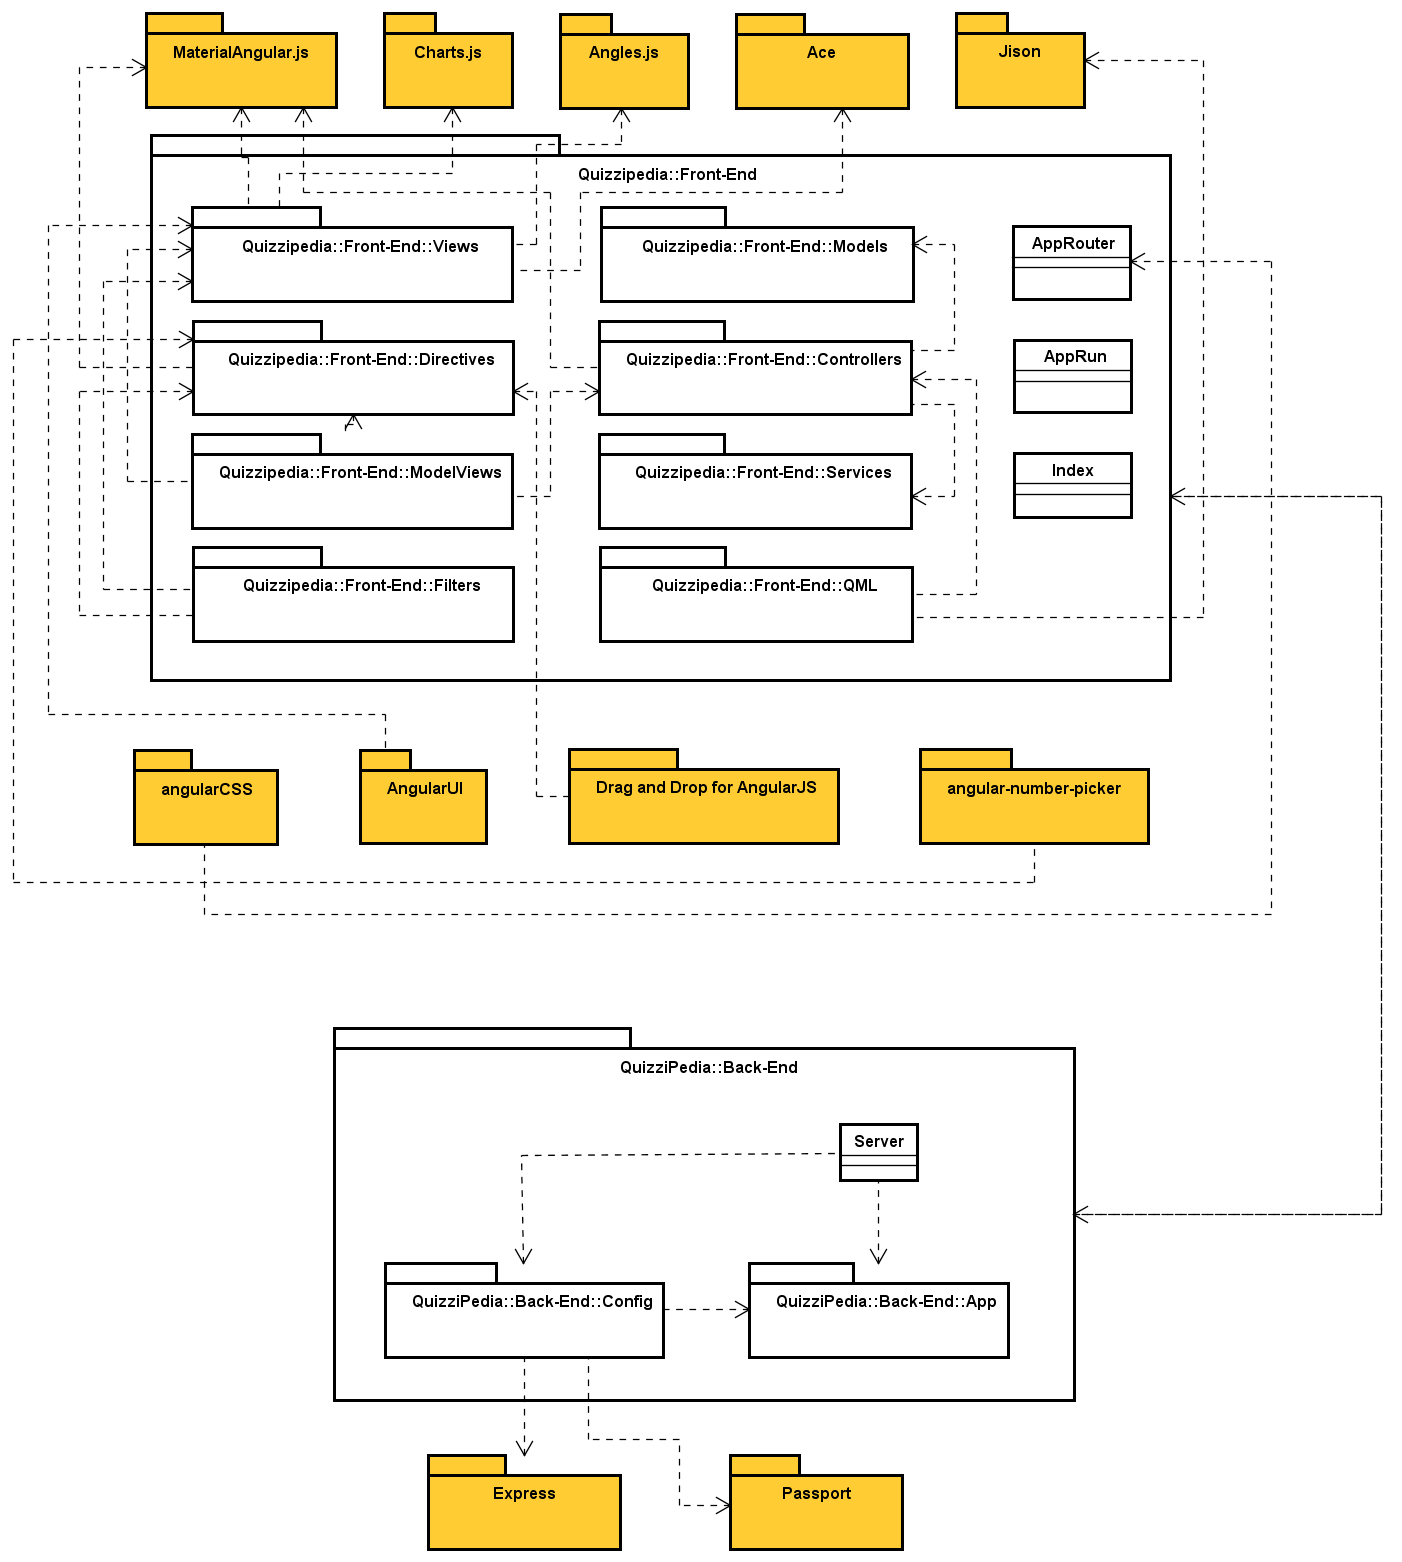
\includegraphics[scale=0.35]{UML/Package/QuizziPedia.png}
	\caption{Architettura}
\end{figure}
\FloatBarrier
\begin{itemize}
	\item \textbf{Descrizione}: architettura ad alto livello dell'applicazione \progetto. Data la natura dell'applicazione, si è scelto di utilizzare come \textit{design pattern\ped{G}} architetturale l'\textit{MVC\ped{G}}, e di dividere le funzionalità in Front-End e Back-End. La parte Front-End, sviluppata secondo il \textit{design pattern\ped{G}} \textit{MVVM\ped{G}}, si occupa principalmente della presentazione a video dei contenuti e dell'interazione con l'utente; la parte Back-End, sviluppato secondo i \textit{design pattern\ped{G}} \textit{Observer\ped{G}} e \textit{Chain-of-responsability\ped{G}}, si occupa invece di elaborare i dati e le azioni che l'utente immette e di dialogare col database;
	\item \textbf{Packages contenuti}:
	\begin{itemize}
		\item \texttt{QuizziPedia::Front-End}: \textit{package\ped{G}} contenente i \textit{packages\ped{G}} che compongono il Front-End;
		\item \texttt{QuizziPedia::Back-End}: \textit{package\ped{G}} contenente i \textit{packages\ped{G}} che compongono il Back-End;
	\end{itemize}
	\item \textbf{Classi contenute}:
	\begin{itemize}
		\item \texttt{AppRouter}: classe che gestisce i routes dell'applicazione, utilizza il servizio \$routeProvider per associare ad ogni route un \textit{controller\ped{G}} e una \textit{view\ped{G}}. Viene utilizzata per associare un URL alle varie \textit{view\ped{G}} dell'applicazione;
		\item \texttt{AppRun}: classe che istanza l'applicazione. Viene utilizzata per indicare le dipendenze tra l'applicazione con i \textit{packages\ped{G}} esterni;
		\item \texttt{Index}: \textit{view\ped{G}} generale dell'applicazione. Contiene gli elementi che saranno presenti in ogni pagina dell'applicazione;
		\item \texttt{Server}: classe che avvia il \textit{server\ped{G}}. Nello specifico apre una connessione al database tramite \textit{Mongoose\ped{G}}, invoca il \textit{middleware\ped{G}} \textit{Express\ped{G}} passando un riferimento al database \textit{MongoDB\ped{G}} come parametro in modo  che possa configurarsi con esso, invoca il \textit{middleware\ped{G}} \textit{Passport\ped{G}} ed infine si mette in ascolto su una determinata porta. E' il componente \textit{client\ped{G}} del \textit{design pattern\ped{G}} \textit{Chain of responsibility\ped{G}}. Utilizza i moduli \textit{Mongoose\ped{G}}, \textit{Express\ped{G}}, \textit{Passport\ped{G}};
		Utilizzata per avviare l'applicazione lato \textit{server\ped{G}}. Inizializza, internamente al back-end, la catena di gestione delle chiamate \textit{REST\ped{G}} utilizzando le classi contenute nel \textit{package\ped{G}} \texttt{Routers}.
	\end{itemize}
	\item \textbf{Librerie e framework}:
	\begin{itemize}
		\item \texttt{MaterialAngular.js}: \textit{framework\ped{G}} per lo sviluppo di componenti UI. Espone un insieme di componenti dell'interfaccia utente riutilizzabili, ben collaudati, e accessibili basati sul \textit{Material Design\ped{G}};
		\item \texttt{Charts.js}:  permette di visualizzate otto differenti tipi di grafici, animati, personalizzabili e \textit{responsive\ped{G}};
		\item \texttt{Angles.js}: per utilizzare la libreria Charts.js all'interno dell'ambiente AngularJS, è necessario l'utilizzo della libreria Angles.js;
		\item \texttt{Ace}: editor di codice scritto in JavaScript e può essere facilmente integrato in qualsiasi pagina web e applicazioni JavaScript;
		\item \texttt{Jison}: generatore di parser in codice JavaScript Jison. Prende una \textit{grammatica context-free\ped{G}} come input e restituisce un file JavaScript in grado di analizzare il linguaggio descritto da quella grammatica. È quindi possibile utilizzare lo script generato per analizzare gli ingressi e di accettare, rifiutare o eseguire azioni in base all'ingresso;
		\item \texttt{AngularCSS}: libreria che permette di ottimizzare il livello di presentazione delle applicazioni in singola pagina con fogli di stile che si iniettano in modo dinamico in base alle esigenze. Resta in ascolto di eventi di modifica, aggiunge il CSS definito sul percorso attuale e rimuove il CSS dal percorso precedente;
		\item \texttt{AngularUI}: libreria per la gestione dei componenti grafici;
		\item \texttt{Drag and Drop for AngularJS}: libreria che permette l'operazione di drag and drop all'interno dell'ambiente AngularJS;
		\item \texttt{angular-number-picker}: direttiva che permette la raccolta di numeri tramite pulsante su / giù, invece di digitarli;
		\item \texttt{Express}: web application \textit{framework\ped{G}} per Node.js. Mette a disposizione numerosi metodi HTTP, il supporto per connect \textit{middleware\ped{G}} e consente di realizzare rapidamente interfacce per la programmazione; richiede moduli Node di terze parti per applicazioni che prevedono l'interazione con le basi di dati;
		\item \texttt{Passport}: \textit{middleware\ped{G}} per Node.js che permette l'autenticazione, in modo sicuro, ad una applicazione web, tramite username e password. 
	\end{itemize}
\end{itemize}
